\documentclass[12pt, openany, oneside, a4paper, english, brazil]{abntex2}   % Padrão Abntex2

%***************************** PACOTES *********************************** %
%\usepackage[within=none]{newfloat}
\usepackage[utf8]{inputenc}		     % Codificacao do documento (conversão automática dos acentos)


%	Fonte
\usepackage[T1]{fontenc}		   	 % Selecao de codigos de fonte.
\usepackage[brazil]{babel}
\usepackage{lmodern}			     % Usa a fonte Latin Modern

%	Matemático e Gráfico
\usepackage{float}
\usepackage{graphics,graphicx}	     % pacotes para inserir figuras .eps ou .jpg
\graphicspath{{figuras/}}            % pasta de figuras
\usepackage{amssymb}           		 % pacote para fontes e simbolos matemáticos
\usepackage{longtable}          	 % possibilita inserir grandes tabelas
\usepackage{makecell}                % possibilita pular linhas nas tabelas
\usepackage{xcolor,colortbl,multirow} % permite textos e tabelas com cores
\usepackage{amsmath}           		 % pacote para equações
\usepackage{epstopdf}
\usepackage{ragged2e}
\usepackage{listings}
%\lstset{numbers=left, numberstyle=\tiny, stepnumber=1, numbersep=5pt, basicstyle=\scriptsize ,frame=tbrl}
\usepackage{etoolbox}
\usepackage{multicol}
% \usepackage{caption}
% \usepackage{subcaption}
\usepackage[position=b,singlelinecheck=on]{subfig}

\floatstyle{plaintop}
\newfloat{quadro}{htbp}{loq}
\floatname{quadro}{Quadro}

\makeatletter
\patchcmd{\listof}% <cmd>
{\float@listhead}% <search>
{\@namedef{l@#1}{\l@table}\float@listhead}% <replace>
{}{}% <success><failure>
\makeatother

%\makeatletter
%\renewcommand*{\float@listhead}[1]{%
%	\@ifundefined{chapter}{%
%		\section*{#1}%
%		\addcontentsline{toc}{section}{#1}%
%	}{%
%	\chapter*{#1}% 
%	\addcontentsline{toc}{chapter}{#1}%
%}%
%\@mkboth{\MakeUppercase{#1}}{\MakeUppercase{#1}}%
%}
%\makeatother




%\DeclareFloatingEnvironment{quadro}[Quadro][Lista de quadros]
%\DeclareCaptionType{quadro}[Quadros][Lista de quadros]


% % % % % % % % % % % % % % % % % % % %

\definecolor{codegreen}{rgb}{0,0.6,0}
\definecolor{codegray}{rgb}{0.5,0.5,0.5}
\definecolor{codepurple}{rgb}{0.58,0,0.82}
\definecolor{backcolour}{rgb}{0.95,0.95,0.92}

%\definecolor{verde}{rgb}{0,0,0}

\lstdefinestyle{mystyle}{
	backgroundcolor=\color{backcolour},   
	commentstyle=\color{codegreen},
	keywordstyle=\color{magenta},
	numberstyle=\tiny\color{codegray},
	stringstyle=\color{codepurple},
	basicstyle=\footnotesize,
	breakatwhitespace=false,         
	breaklines=true,                 
	captionpos=b,                    
	keepspaces=true,                 
	numbers=left,                    
	numbersep=5pt,                  
	showspaces=false,                
	showstringspaces=false,
	showtabs=false,                  
	tabsize=2
}

\lstset{style=mystyle}

%	Estrutural
\usepackage{url}
\usepackage{threeparttable}     	 % permite a inserção de notas de rodapé nas tabelas
\usepackage{lscape}             	 % orientação de página LANDSCAPE
\usepackage{pifont}             	 % acrescenta símbolos diferentes.
%\usepackage{cmap}					 % Mapear caracteres especiais no PDF	
\usepackage{lastpage}				 % Usado pela Ficha catalográfica
\usepackage{indentfirst}			 % Indenta o primeiro parágrafo de cada sessão.



% Pacotes de citações
\usepackage[brazilian,hyperpageref]{backref}	 % Paginas com as citações na bibl
\usepackage[num]{abntex2cite}	% Citações padrão ABNT numerica
\citebrackets[]     
% remover bordas dos links
\hypersetup{
    colorlinks,
    linkcolor={black},
    citecolor={black},
    urlcolor={black}
}

\usepackage[round]{natbib}
\bibliographystyle{plainnat}
 % resto dos pacotes Latex
%\usepackage[english]{style/UFSC-ECA-Monograph} % personalização da ABNTEX2 para escrita em inglês
\usepackage[portuguese]{style/UFSC-ECA-Monograph} % personalização da ABNTEX2 para escrita em português


%---------------------------------------------------------------
%--------- DADOS BÁSICOS DO TRABALHO (Preencher todos) ---------
%---------------------------------------------------------------


\titulo{Bancada Experimental para Aquisiçao de Coeficientes Aerodinamicos de VANTs sem Tunel de Vento}   % Título do Trabalho em Português
\tituloingles{Experimental bench for aquisition of aerodynamic coefficients of UAVs without wind-tunnel}   % Título do Trabalho em Inglês

\palavraschave{1. VANT. 2. Bancada. 3. Coeficientes.}  % 5 palavras-chave
\keywords{1. UAV. 2. Bench. 3. Coefficients.}   % 5 palavras-chave para resumo em inglês

\DEELautor{Rafael}{Araujo Lehmkuhl} % Aluno autor do trabalho

\curso{Engenharia Mecânica}												
\orientador{Prof. Dr. Amir Antonio Martins de Oliveira Junior}  % Professor Orientador membro da banca 

\membrob{Prof. Dr. XXX1}   % Professor membro da banca 
\membroc{Prof. Dr. XXX2}   % Professor membro da banca

\local{Florianópolis}   % Cidade da instituição
\data{2019}        % Ano de realização


%--------------------------------------------------------------------------------------------



\begin{document}
% Seleção automática do idioma, não alterar
\ifx\isenglish\undefined
    \selectlanguage{brazil}
\else
    \selectlanguage{english}
\fi

% Texto da Dedicatória (OBS: dedicatória é opcional)
% Caso não queira inserir, deixe em branco ( \dedicatoria{} )
\DEELdedicatoria{Dedico este trabalho a todos aqueles que, de alguma forma,\\ auxiliaram para a concretização desta etapa, em especial aos meus pais, que sempre me proporcionaram a melhor educação que eu poderia ter e a equipe Céu Azul Aeronaves, responsável por manter acesa minha paixão pela engenharia.\\}  
    
% Texto dos Agradecimentos (OBS: Agradecimentos é opcional)
% Caso não queira inserir, deixe em branco ( \agradecimentos{} )
\DEELagradecimentos{Agradeço a meu pai, minha mãe e a minha ex, que me aguentou quase até o final da elaboraçao deste trabalho.} 
    
                                  
% Texto da Epígrafe (OBS: Epígrafe é opcional)
% Caso não queira inserir, deixe em branco ( \epigrafe{} )
\DEELepigrafe{\textit{"Tem que ver isso ai, talkei?."} \\ (BOLSONARO, Jair)} 
\DEELepigrafe{\textit{"Essa pica não é mais minha. Essa pica agora é do aspira."} \\ (FÁBIO, Capitão)}
\DEELepigrafe{\textit{"Bora bar."} \\ (MEMBRO DO AERO, Qualquer)} 
\DEELepigrafe{\textit{"Pau no cu de quem não gostou."} \\ (LEHMKUHL, Rafael A.)} 
    

% Texto do Resumo (OBS: Resumo é Obrigatório)
\DEELresumo{Resumo em português.} 
     
% Texto do Abstract (OBS: Abstract é Obrigatório)
\DEELabstract{Abstract in english.} 
    



%%%%%%%%%%%%%%%%%%%%%%%%%%%
%% Elementos Pré-Textuais%%
%%%%%%%%%%%%%%%%%%%%%%%%%%%
\ElementosPreTextuais
% Insere todos os elementos Pré-Textuais listados (capa, folha de rosto, ...)
    % capa                   % Obrigatório
    % folhaderosto           % Obrigatório
    % folhaaprovacao         % Obrigatório
	% dedicatoria            % Opcional
	% agradecimentos         % Opcional
    % epigrafe               % Opcional
    % resumo                 % Obrigatório
    % abstract               % Obrigatório
\
%\newpage
%--------Lista de figuras--------
\ListaDeFiguras 
%--------Lista de tabelas--------
\ListaDeTabelas 
%--------Lista de Siglas e Abreviaturas--------
%----------Lista de Acronimos --------------------------------
\ifx\isenglish\undefined
\pretextualchapter{Lista de Siglas e Abreviaturas}
\else
\pretextualchapter{Acronyms}
\fi


%\renewcommand{\baselinestretch}{2} %espaçamento entre linhas (por definicçào, no espABNT é 2)
\begin{tabbing}
xxxxxxxxxxx \= xxxxxxxxxxxxx \kill
\textsc{ROS}            \> \textit{Robot Operating System}\\
\textsc{UFSC} \> \textit{Universidade Federal de Santa Catarina}\\
\end{tabbing}

%\addcontentsline{toc}{chapter}{Lista de Siglas e Abreviaturas}
   
%--------Lista de Simbolos e Notação--------
%\include{list_simbolos} 
%--------Sumário-------
\Sumario


%%%%%%%%%%%%%%%%%%%%%%
%%Elementos Textuais%%
%%%%%%%%%%%%%%%%%%%%%%
\textual 
\chapter{Introdução}\label{chp:intro}

Com a recente diminuição do custo das plataformas de processamento e sensoriamento embarcado [X] um novo ramo de mercado surgiu ao redor do desenvolvimento de VANTs [x].

Ainda que os avanços na tecnologia de baterias tenha permitido que este mercado surgisse, sua baixa densidade de potencia[X] exige que os projetos de VANTs sejam altamente otimizados em relação ao consumo energético.

Um problema frequente em projetos aeronáuticos, porém, é a incerteza quanto aos dados aerodinâmicos dos diversos componentes que compõem a aeronave. A resolução deste problema é abordada em geral de três maneiras: estimativas teóricas [X], simulação fluidodinâmica [X] e experimentação, possuindo cada um destes suas vantagens e desvantagens.

As estimativas teóricas em geral se encontram no projeto como método inicial de avaliação. A vantagem desta se dá pela vasta literatura disponível e por consistir na aplicação de fórmulas (em geral) simples. A desvantagem está na incerteza sobre a exatidão do resultado, isto é, não se sabe o quanto o mesmo esta próximo da realidade, ou mesmo se o valor é subestimado ou superestimado.

A simulação é uma alternativa muito utilizada, e sua vantagem se dá na maior exatidão dos resultados quando o modelo e os parâmetros de simulação já são bem conhecidos e comportados para a geometria estudada. O problema principal deste método se encontra na maior dificuldade de emprego, pois se limita a modelos que já tenham sido validados contra resultados experimentais. Para geometrias pouco estudadas, com parâmetros de simulação desconhecidos, corre-se o risco inclusive de se obter resultados ordens de grandeza afastados da realidade[X].

Por ultimo, a experimentação consiste em preparar um modelo físico semelhante ao projetado e ensaia-lo em um escoamento com as características desejadas. A dificuldade de emprego deste em geral é maior que a dos primeiros por exigir um trabalho de construção bem executado e equipamentos de medição com elevada precisão. Estas características fazem com que a experimentação tenha um custo elevado, muito diferente dos dois primeiros métodos, que tem custo praticamente nulo. Sua vantagem, porém, se dá no fato de que a certeza sobre os valores encontrados em geral é muito maior. Caso o teste tenha sido executado da maneira correta, os equipamentos de medição tenham precisão conhecida e sejam respeitadas as premissas do modelo, chega-se num resultado que pode ser tomado como real dentro de um intervalo de incerteza do equipamento de medição, isto é, diferente dos dois métodos anteriores, onde o resultado encontrado pode não corresponder com a realidade, neste existe uma faixa de certeza sobre o resultado.

\section{Sobre o projeto}

O principal problema do método experimental é a necessidade de equipamento especializado, e o método mais comum envolve a caracterização do modelo construído (em escala ou não) em um túnel de vento, com as forças medidas através de uma balança de precisão [X]. Túneis de vento, contudo, são equipamentos grandes e caros, e não disponíveis na maioria das universidades brasileiras. Túneis pequenos, como o da UFSC, são mais comuns porém não apresentam a possibilidade de medição de esforços aerodinâmicos em geometrias mais sofisticadas, devido a alta interferência no escoamento gerada pelas paredes do túnel. Componentes como asas, dispositivos de ponta de asa, conjuntos moto-propulsores, entre outros, que possuem grande relevância nos cálculos aerodinâmicos, acabam não podendo ter seu comportamento caracterizado nessas universidades.

\begin{figure}[!ht]
    \centering
    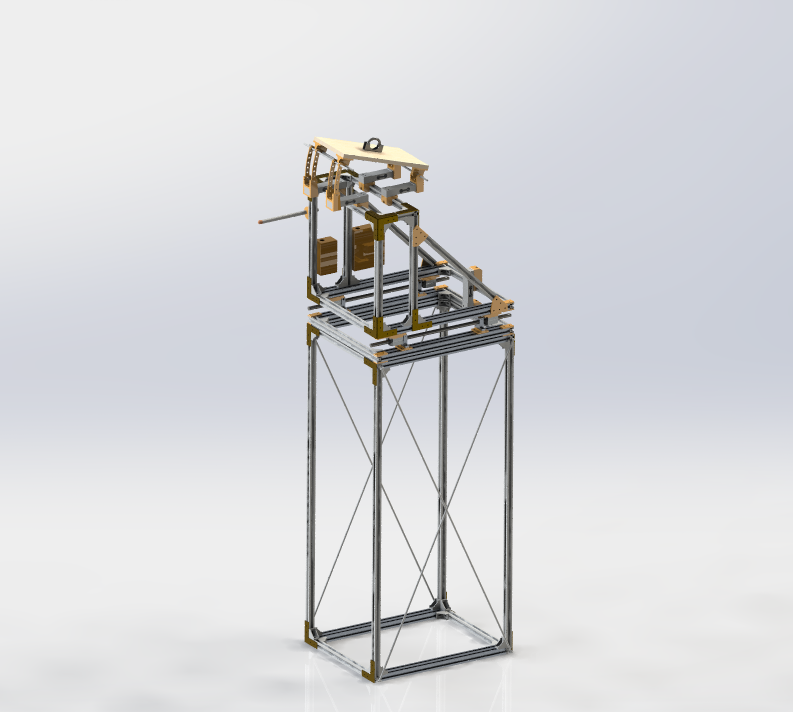
\includegraphics[width=.8\linewidth]{figuras/renders/perspectiva_sem_asa_com_pitot.png}
    \caption{Renderização da bancada modelada no software Solidworks 2016\cite{autor}.}
    \label{fig:placeholder}
\end{figure}

\begin{figure}[!ht]
    \centering
    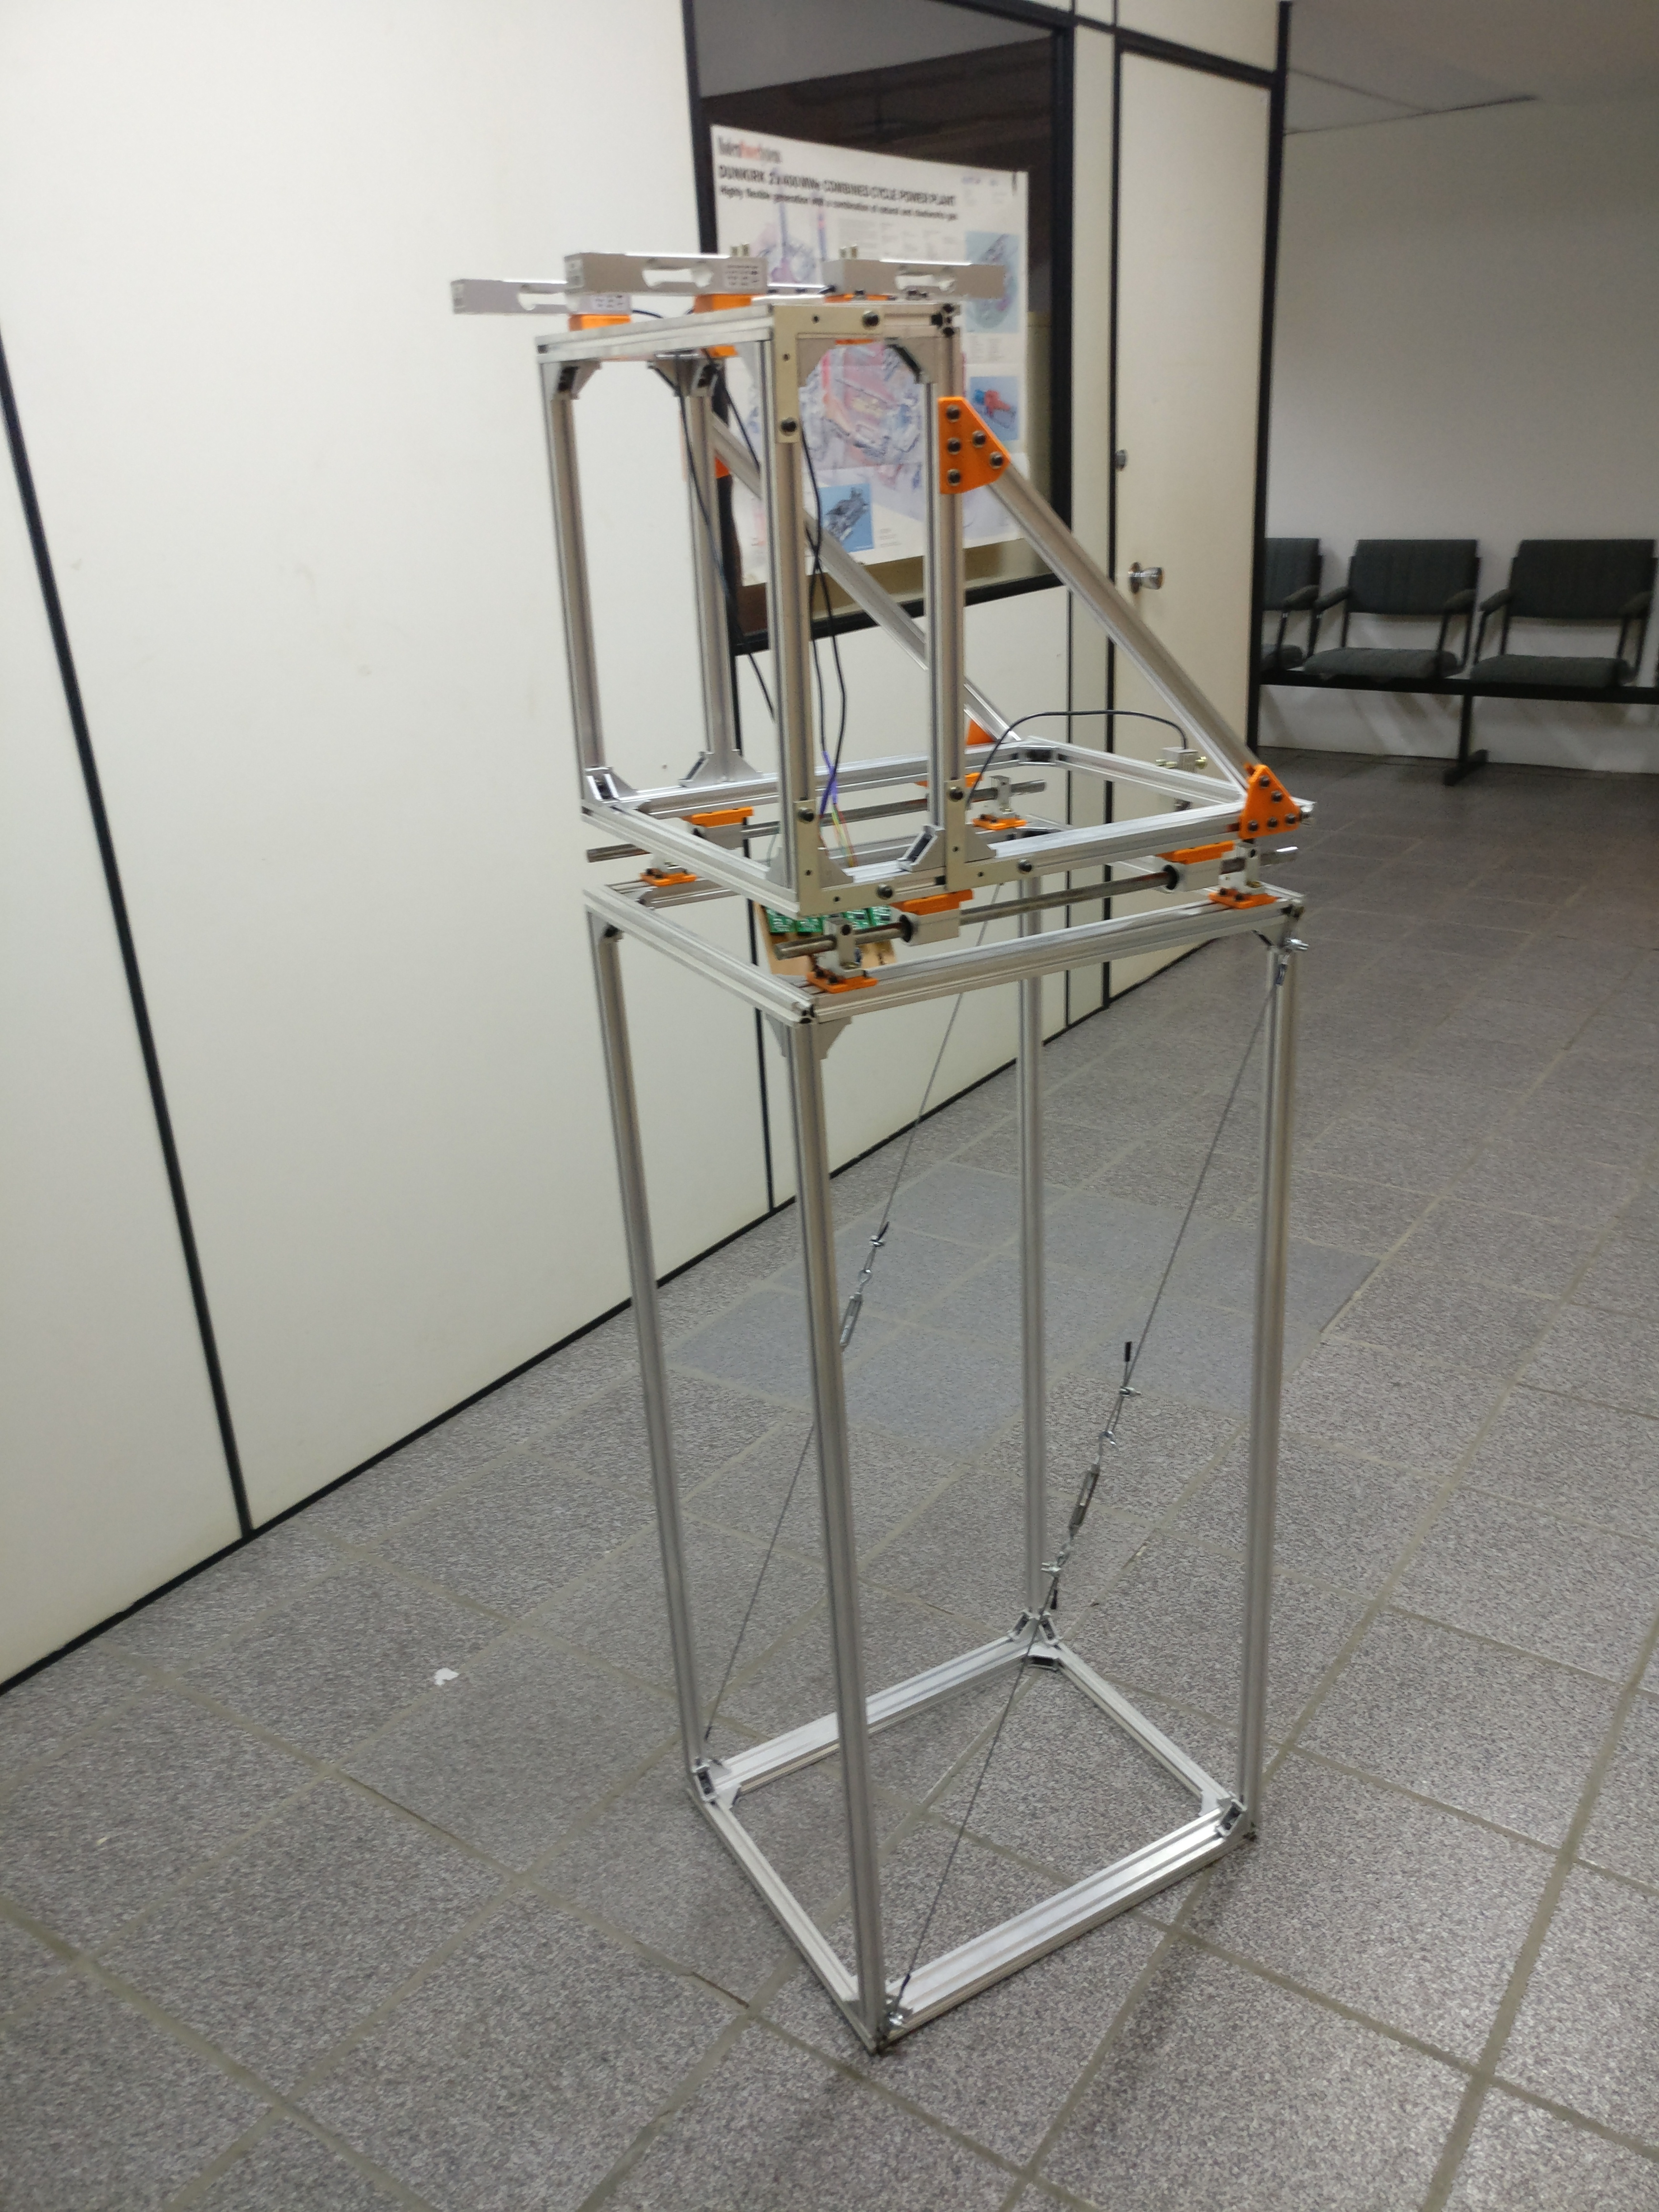
\includegraphics[width=.8\linewidth]{figuras/construcao/bancada_inteira.jpg}
    \caption{Foto da bancada construída\cite{autor}.}
    \label{fig:placeholder}
\end{figure}

A proposta deste trabalho consiste no projeto e análise de uma bancada para medição de esforços aerodinâmicos sem túnel de vento, a ser utilizada para a caracterização aerodinâmica de componentes de VANTs. Tal bancada consiste de células de carga, tubos de pitot e outros sensores, e é embarcada em um veiculo automotor, que ao ser movimentado faz com que um escoamento surja sobre o componente a ser experimentado.

\section{Objetivo geral}

Desenvolvimento de uma bancada de baixo custo para caracterização aerodinâmica de componentes de VANTs, visando a eliminação ou minimização da necessidade de um túnel de vento.
 % Texto do cap1.tex
\chapter{Revisão de Literatura}\label{chp:rev}

Bancada semelhante já foi construída pela NASA para estudos aerodinâmicos da aeronave LEAPtech [6], e seus resultados comparados aos simulados em computador [7].


\begin{itemize}
    \item Revisao de aerodinamica
    \item Revisao de metrologia
    \item Projeto Bancada 1.0
\end{itemize} % Texto do cap2.tex
\chapter{Metodologia}\label{chp:met}

\section{Projeto}

\begin{itemize}
    \item Levantamento das necessidades
    \item Levantamento das possiveis solucoes
    \item Projeto da bancada 1.0
    \item Levantamento dos problemas da 1.0
    \item Levantamento das possiveis soluçoes para a 1.0
\end{itemize}

\subsection{Necessidades}

O cliente do presente projeto é a equipe Céu Azul Aeronaves, que representa anualmente a UFSC na competiçao SAE Brasil Aerodesign.

O objetivo da bancada proposta neste trabalho é o de medir os coeficientes aerodinamicos (de sustentaçao, arrasto e momento) em diversas geometrias expostas a um escoamento de ar relativamente bem comportado. Tais geometrias incluem componentes de aeronaves do tipo VANT, como asas, profundores, fuselagens e outros dispositivos. Além disso, o uso para a mediçao de curvas de empuxo dinamico (isto é, o empuxo medido para diferentes velocidades) de motores é desejado.

Tal bancada deve possuir rigidez suficiente para que suas mediçoes sejam consistentes no tempo. Deve ser possivel também prende-la a caçamba de uma camionete ou ao rack de um carro comum, de modo a facilitar sua instalaçao sem grande dificuldade.

Levando em conta que a equipe sofre de alta rotatividade de membros, e nem sempre é possivel garantir que existirao pessoas capacitadas a trabalhar neste projeto, é importante que a bancada em questao seja entregue na forma de um "produto final", isto é, funcione sem a necessidade de conhecimento de suas intricidades, com pouco mais que um manual de instruçoes e consideraçoes para seu uso.

Da mesma forma que o uso da bancada deve ser facilitado, também deve ser assim o uso dos dados fornecidos por ela. Idealmente se deseja que a mesma entregue os coeficientes finais, ja processados, assim como suas incertezas de mediçao.

\subsection{Consideraçoes e estimativas}

Assume-se para o presente projeto que o escoamento de ar que alcança a geometria analisada tem direçao relativamente estavel (e aproximadamente paralela ao deslocamento do veiculo) e velocidade praticamente constante para pequenos trechos a serem analisados. Oscilaçoes da ordem de 10\% na velocidade sao esperadas e podem ser facilmente mensuradas através de sensoriamento adequado (tupo de pitot e GPS, por exemplo). 

\begin{figure}[!ht]
    \centering
    \includegraphics[width=.8\linewidth]{figuras/placeholder.png}
    \caption{FIGURA COM ANGULO DE ESCOAMENTO INDUZIDO PELO VEICULO\cite{autor}.}
    \label{fig:vehicle-angle}
\end{figure}

É possivel também que a carroceria do veiculo induza um angulo diferente de zero ao escoamento que chega a bancada (ver \prettyref{fig:vehicle-angle}). Se este angulo for de pequena ordem (menor que 15 graus) um pitot de multiplas tomadas pode ser utilizado para medi-lo e normalizar os dados em um pos-processamento. Grandes desvios de direçao ou velocidades muito instaveis provavelmente tornarao o processamento dos dados dos testes impeditivo.

\begin{figure}[!ht]
    \centering
    \includegraphics[width=.8\linewidth]{figuras/placeholder.png}
    \caption{FIGURA MOSTRANDO FORCA RADIAL INDUZIDA POR PISTA CURVA\cite{autor}.}
    \label{fig:placeholder}
\end{figure}

\begin{figure}[!ht]
    \centering
    \includegraphics[width=.8\linewidth]{figuras/placeholder.png}
    \caption{FIGURA MOSTRANDO FATOR DE CARGA SENTIDO EM OSCILACOES\cite{autor}.}
    \label{fig:placeholder}
\end{figure}

Assume-se também que existem obstaculos na pista de teste (tais como buracos e pequenas elevaçoes), mas que de forma geral o teste sera conduzido em pistas relativamente retas e planas, de modo que nao existam vibraçoes constantes ou aceleraçoes radiais a serem modeladas no sistema. Pequenas oscilaçoes podem ser medidas por dispositivos adequados e levadas em conta no pos-processamento.

Para os projetos mecanico e eletronico considera-se as possiveis situaçoes a serem mensuradas:


\begin{itemize}
    \item Caracterizaçao de aeronave completa com 200N de sustentaçao, 50N de arrasto e XXXN de Momento
    \item Caracterizaçao de conjunto motopropulsor com 60N de empuxo estatico
    \item Escoamentos com velocidade de até 25m/s
    \item Fatores de carga na bancada de até 2g
\end{itemize}

A camionete a ser utilizada nos testes é do modelo Fiat Strada 2010, tendo a caçamba uma altura de XXXm e o teto do carro elevando-se XXXm além da altura da caçamba.

\subsection{Soluçao proposta}

\begin{figure}[!ht]
    \centering
    \includegraphics[width=.8\linewidth]{figuras/placeholder.png}
    \caption{ESQUEMATICO DA BANCADA + TORRE\cite{autor}.}
    \label{fig:placeholder}
\end{figure}

A soluçao proposta consiste em uma bancada sensoriada montada sobre uma torre que a coloque na altura desejada. As forças na bancada sao sensoriadas com quatro celulas de cargas verticais e uma ou mais celulas de carga horizontais. As celulas horizontais permitem a mediçao do arrasto, o somatorio das celulas verticais permitem a mediçao da sustentaçao, a diferença entre as celulas frontais e traseiras permite a mediçao do momento de picada (pitch) e a diferença entre as celulas da esquerda e da direita permite a mediçao do momento de rolagem (roll).

\begin{figure}[!ht]
    \centering
    \includegraphics[width=.8\linewidth]{figuras/placeholder.png}
    \caption{ESQUEMATICO COM DISPOSICAO DAS CELULAS\cite{autor}.}
    \label{fig:placeholder}
\end{figure}

Ainda na bancada serao instalados ao menos um tubo de pitot e um pitot de multiplas tomadas. Ambos serao colocados em escoamento livre, proximos ao teto da bancada, de modo a se aproximar da altura da geometria a ser analisada. O sistema deve comportar ainda a adiçao de novos sensores de forma a se caracterizar o escoamento em outros pontos de interesse. Para a mediçao da velocidade absoluta do carro sera utilizado um sistema GNSS acoplado a bancada.

Para a mediçao do fator de carga vertical, assim como da temperatura e pressao do ar, uma IMU com acelerometro, barometro e termometro sera instalada bancada.

\begin{figure}[!ht]
    \centering
    \includegraphics[width=.8\linewidth]{figuras/placeholder.png}
    \caption{FOTO DA IMU\cite{autor}.}
    \label{fig:placeholder}
\end{figure}

Num primeiro momento foi levantada a possibilidade de se utilizar um computador portatil como central de comando da bancada, porém isto poderia tornar o uso dificultado, ja que em geral estes computadores possuem baterias que permitem poucas horas de uso continuo, limitando o tempo de execuçao de teste, além de serem relativamente grandes e pouco praticos de se utilizar dentro do carro. De forma a facilitar o uso da bancada todo o comando do sistema sera realizado através de um aplicativo para celular. Nele sera possivel acompanhar o estado da bancada, controlar o teste, inserir informaçoes para avaliaçao posterior, assim como acompanhar as mediçoes em tempo real, de modo a identificar possiveis problemas de forma rapida.

Sera desenvolvido ainda um software de tratamento e analise de dados com interaface grafica e uso facilitado, este sim a ser utilizado em computador, devido a maior flexibilidade do mesmo para trabalhos mais longos.

\section{Projeto Mecânico}

Para o projeto mecanico foram levantadas as seguintes necessidades:

\begin{itemize}
    \item Facilidade construtiva, de forma a tornar rápida a construção e manutenção da bancada
    \item Leveza, de modo a não se criar uma barreira quanto ao uso da mesma
    \item Baixo arrasto aerodinâmico, a fim de diminuir a influência da estrutura nas medições
    \item Rigidez, para que as forças e momentos medidos sejam realmente os modelados
    \item Baixo custo
\end{itemize}

Uma soluçao que responde de forma positiva a maioria dessas necessidades é a de uma estrutura composta de perfis extrudados de aluminio. Este tipo de estrutura é muito comum de ser encontrada em laboratorios ou fabricas, sendo comumente utilizada para a construçao de bancadas experimentais e estaçoes de trabalho.

\begin{figure}[!ht]
    \centering
    \includegraphics[width=.8\linewidth]{figuras/placeholder.png}
    \caption{FOTO DO PERFIL DE ALUMINIO\cite{autor}.}
    \label{fig:placeholder}
\end{figure}

O contra desta estrutura fica pelo provavel alto arrasto aerodinamico. Este problema porem pode ser contornado posteriormente carenando-se a estrutura, semelhante ao que se faz em aeronaves. Ainda assim este arrasto, com ou sem carenagem, deve ser levado em conta nos testes e a maneira levantada de se mensurar esta grandeza é realizar os testes com a bancada sem geometria acoplada, medindo-se assim o arrasto aerodinamico da propria bancada e descontando este valor das mediçoes posteriores.

De modo a se medir o arrasto, duas soluçoes sao possiveis: 

\begin{enumerate}
    \item Colocar uma celula de carga horizontal e dar liberdade de mvoimento para a bancada no eixo X
    \item Ter como unicas restriçoes no eixo X células de carga
\end{enumerate}

\begin{figure}[!ht]
    \centering
    \includegraphics[width=.8\linewidth]{figuras/placeholder.png}
    \caption{ESQUEMATICO DAS SOLUCOES 1 E 2\cite{autor}.}
    \label{fig:placeholder}
\end{figure}

Devido ao fato de que a segunda soluçao exigiria ao menos tres celulas de carga e as colocaria como componentes estruturais (ja que nao existiria outra ligaçao estrutural entre a parte inferior e superior da bancada) a primeira opçao foi escolhida.

Para dar liberdade de movimentaçao no eixo X um conjunto de guias lineares e fixaçoes rolamentadas foi escolhido, devido a seu baixo atrito e baixo custo. O contra da soluçao com apenas uma celula de carga se da justamente devido a existencia desta força de atrito das guias no eixo X, que a principio existe e nao é medida. Esta força pode porem ser avaliada num primeiro momento, em laboratorio, e compensada posteriormente.
    
\section{Projeto Eletrônico}

Para o sistema eletronico da bancada, tomou-se como ponto de partida a telemetria T2016, desenvolvida pela equipe Céu Azul inicialmente para utilização nos projetos da classe Advanced.

Tal sistema consiste de um computador central, modelo Raspberry Pi 3 B+, rodando um sistema operacional Linux, com sensores conectados como perifericos. Entre os sensores ja disponiveis na equipe estavam:

\begin{itemize}
    \item Tubos de pitot com transdutores MPVX7002DP
    \item GNSS modelo uBlox neo-6m
    \item IMU modelo GY85, com acelerometro de 3 eixos, giroscopio de 3 eixos, magnetometro de 3 eixos, barometro e termometro
\end{itemize}

Alem destes sensores o sistema possuira um par de rádios seriais de 433MHz, que pode ser utilizdo para transmissão dos dados em tempo real para o celular, comunicando a bancada com o aplicativo controlado pelo operador.

Para a mediçao das forças na bancada foi necessaria a aquisiçao de células de carga e transdutores de célula de carga. Devido ao baixo custo optou-se por células sem marca. Esta decisao implica contudo num custo extra de tempo para a caracterizaçao das células.

Para a transduçao dos dados da celula (de resistencia para tensao e posteriormente para força) foram adquiridos módulos HX711. Estes modulos sao bastante comuns no mercado e implementam num mesmo CI a alimentaçao e leitura da ponte de wheatstone, alem da transformaçao em dados digitais. A maior vantagem deste CI é provavelmente a alimentaçao integrada da ponte de Wheatstone, que é no caso ja estabilizada e filtrada, resultando em uma alta relaçao sinal-ruido. Em geral essa alimentaçao acontece em circuitos discretos separados do CI de leitura, e acabam resultando numa pior relaçao sinal-ruido.

\section{Projeto de Software Embarcado}

O software que roda de forma embarcada na plataforma central consiste em uma serie de modulos escritos em Python com funçoes desmembradas. Entre as funçoes necessarias no software destacam-se:

\begin{itemize}
    \item Aquisiçao de dados dos sensores
    \item Parseamento dos dados para padrao comum
    \item Transmissao serial de dados via radio
    \item Recebimento e interpretaçao de comandos externos
    \item Gravaçao dos dados no sistema
    \item Coordenaçao e sincronia dos processos anteriores
\end{itemize}

A figura X mostra a arquitetura do software divida em seus varios modulos.

\begin{figure}[!ht]
    \centering
    \includegraphics[width=.8\linewidth]{figuras/placeholder.png}
    \caption{ESQUEMATICO DO SOFTWARE EMBARCADO\cite{autor}.}
    \label{fig:placeholder}
\end{figure}

Este software ja existia em versao primaria na plataforma T2016 e foi refatorado para uso na nova plataforma, permitindo que suas funçoes fossem extendidas. A totalidade das mudanças compreendidas por este trabalho pode ser vista no repositorio Git do projeto [X]. 

\section{Projeto de Software de Analise}

O software de analise de dados tem por funçao receber os dados "crus" gerados pela bancada e entregar dados uteis processados, com suas devidas incertezas estimadas.

Entre as funçoes desejadas neste software estao:

\begin{itemize}
    \item Apresentar uma interface amigavel para uso facilitado
    \item Receber os dados "crus"
    \item Filtrar cada dado conforme especificaçoes previas ou personalizadas pelo usuario
    \item Apresentar os dados crus e processados na forma de graficos
    \item Permitir interaçao do usuario com os dados
    \item Exportar os dados em formato util, seja na forma textual, em planilhas ou mesmo diretamente como graficos
\end{itemize}

A figura X mostra a arquitetura deste software.

\begin{figure}[!ht]
    \centering
    \includegraphics[width=.8\linewidth]{figuras/placeholder.png}
    \caption{ESQUEMATICO DO SOFTWARE DE ANALISE\cite{autor}.}
    \label{fig:placeholder}
\end{figure}

\section{MVP}

Para validar a ideia desta bancada foi proposto um MVP que possuise as principais caracteristicas da soluçao proposta, mas que pudesse ser construido com materiais ja disponiveis pela equipe.

Do ponto de vista de projeto mecanico, esta primeira versao da bancada teve sua estrutura construida em madeira, utilizou corrediças de gaveta para dar liberdade de movimento no eixo X e usava como torre uma estrutura de aço. A escolha por estas soluçoes se deu pela ja disponibilidade das mesmas na equipe Céu Azul.

Do ponto de vista de projeto eletronico todos os componentes ja estavam presentes, com exceçao do pitot de multiplos angulos, das celulas de carga e dos modulos HX711, sendo estes ultimos dois adquiridos.

Do ponto de vista de software o aplicativo para controle da bancada foi desenvolvido de forma preliminar enquanto o software de tratamento e analise de dados ainda nao existia.

As fotos a seguir mostram o MVP finalizado.

\begin{figure}[!ht]
    \centering
    \includegraphics[width=.8\linewidth]{figuras/placeholder.png}
    \caption{FOTO DA BANCADA 1.0 - 1\cite{autor}.}
    \label{fig:placeholder}
\end{figure}

\begin{figure}[!ht]
    \centering
    \includegraphics[width=.8\linewidth]{figuras/placeholder.png}
    \caption{FOTO DA BANCADA 1.0 - 2\cite{autor}.}
    \label{fig:placeholder}
\end{figure}

Foi realizada uma serie de testes com esta bancada, entre eles o de mediçao de forças aerodinamicas em uma asa, de mediçao do empuxo dinamico em motor e de mediçao do momento causado pelo acionamento de superficies de comando (ailerons) em uma asa. O procedimento destes testes e seus resultados esta detalhado em [artigo_bancada_1]. Destacam-se aqui as principais conclusoes levantadas por [artigo_bancada_1]:

\begin{itemize}
    \item ponto1
    \item ponto2
    \item ponto3
\end{itemize}

Fica claro portanto que o MVP foi um sucesso no sentido de que provou o funcionamento da bancada proposta, porém possuia problemas estruturais intrinsecos as escolhas para a prototipagem mecanica, e portanto nao demonstrou fidelidade suficiente para seu uso. Além disso, ficaram claros diversos problemas do ponto de vista de praticidade, entre eles:

\begin{itemize}
    \item Aplicativo ainda em estagio inicial, apresentando uma interface pouco intuitiva
    \item Dificuldade para se ajustar o angulo de incidencia do dispositivo testado
    \item Problemas recorrentes de mal-contato elétrico, resultando na perda de baterias inteiras de dados
    \item Pouco controle sobre o estado e funcionamento do computador da bancada
    \item Configuraçao do teste no computador da bancada era realizado modificando-se o script original, o que tornava esta configuraçao bastante suscetivel a erros pelo operador 
    \item Software embarcado (no computador da bancada) pouco organizado, com as estruturas de funcionamento do software altamente entrelaçadas
    \item Falta de sincronia entre os dados das celulas de carga com relaçao aos outros sensores, o que tornava o processamento dos dados um processo bastante massante
    \item Falta de informaçoes sobre o teste no arquivo de gravaçao dos dados, o que fazia com que o operador precisasse recorrer a outros meios para guardar a informaçao sobre o que e como estava sendo feito em cada bateria de testes, causando muitas vezes a perda de informaçao sobre as mesmas
    \item Falta de software para analise dos dados, o que tornava o processo de utilizaçao dos dados gerados pela bancada uma tarefa altamente especializada
\end{itemize}

Estes pontos foram tomados como base para a segunda versao da bancada, detalhada neste texto.

\section{Primeira versao final}

Levando em conta os pontos levantados no MVP deu-se inicio a modelagem e construçao da primeira versao final da bancada.

\subsection{Modelo físico}

COMENTAR SOBRE O MODELO ESTATICO E A CORRECAO DE FALSA SUSTENTACAO

\subsection{Mecanica}

A estrutura da bancada utilizando perfis extrudados em aluminio foi modelada no software Solidworks.

\begin{figure}[!ht]
    \centering
    \includegraphics[width=.8\linewidth]{figuras/placeholder.png}
    \caption{RENDERINGS DA ESTRUTURA DA BANCADA\cite{autor}.}
    \label{fig:placeholder}
\end{figure}

Os perfis de aluminio sao adquiridos em barras de 1 metro de comprimento. A modelagem permitiu assim a definiçao das medidas dos cortes a serem realizados e a otimizaçao do uso das barras.

Utilizando a estimativa de esforços assumida previamente foi desenvolvida a estrutura da bancada realizando-se simulaçoes estruturais no software Ansys Mechanical de modo a se avaliar os deslocamentos maximos da estrutura. Para o projeto decidiu-se por nao permitir deslocamentos verticais maiores que Xmm e deslocamentos horizontais maiores que Xmm. Esta restriçao visa impedir que a deformaçao da bancada induza erros de alinhamento e consequentemente misture as medidas de sustentaçao e arrasto [X].

\begin{figure}[!ht]
    \centering
    \includegraphics[width=.8\linewidth]{figuras/placeholder.png}
    \caption{RENDERING DA SIMULACAO DE ESFORÇOS MECANICOS NA BANCADA\cite{autor}.}
    \label{fig:placeholder}
\end{figure}

As conexoes estuturais foram feitas com cantoneiras planas de aço, garantindo rigidez nas juntas, o que agrega fidelidade na simulaçao (uma vez que nela as juntas sao consideradas rigidas).

Para o encaixe das células de carga na bancada, assim como dos suportes das guias lineares e dos pillow-blocks, foram projetados adaptadores que posteriormente foram produzidos via manufatura aditiva de polímero. Este método de manufatura permitiu a rapida prototipagem dessas peças e acelerou o desenvolvimento do projeto.

\begin{figure}[!ht]
    \centering
    \includegraphics[width=.8\linewidth]{figuras/placeholder.png}
    \caption{FOTO DAS PEÇAS IMPRESSAS - 1\cite{autor}.}
    \label{fig:placeholder}
\end{figure}

\begin{figure}[!ht]
    \centering
    \includegraphics[width=.8\linewidth]{figuras/placeholder.png}
    \caption{FOTO DAS PEÇAS IMPRESSAS - 2\cite{autor}.}
    \label{fig:placeholder}
\end{figure}

\begin{figure}[!ht]
    \centering
    \includegraphics[width=.8\linewidth]{figuras/placeholder.png}
    \caption{FOTO DAS PEÇAS IMPRESSAS - 3\cite{autor}.}
    \label{fig:placeholder}
\end{figure}

Devido a dificuldade na simulaçao de peças produzidas por este processo, que possuem alta anisotropia e grande dispersao nos resultados dependendo da qualidade da impressao, foram realizados testes estruturais estaticos para se garantir que as peças nao falhassem. 

Cabe aqui um adendo de que, para se garantir ainda maior rigidez a bancada como um todo, é de interesse a produçao dessas peças em metal, realizando as devidas modificaçoes para melhor se adequar ao processo de manufatura escolhido.

COMENTAR SOBRE A GUIA LINEAR E SEU MENOR ATRITO E MELHOR ALINHAMENTO

COMENTAR SOBRE OS CABOS DE ACO

COMENTAR SOBRE O AJUSTE DE ANGULO DE INCIDENCIA

\subsection{Eletronica}

Como um dos maiores problemas do MVP foi o de falha no sistema eletronico devido a mal-contato, atençao especial foi dada a esta parte. Duas soluçoes foram levantadas:

\begin{itemize}
    \item Produçao de placas de circuito impresso para o sistema
    \item Utilizaçao de conectores mais robustos
\end{itemize}

Foram produzidas duas PCBs: uma para os transdutores de celula de carga e o Arduino responsavel pela aquisiçao de seus sinais e outra para os transdutores de pressao e o ADC responsavel pela conversao do seu sinal.

\begin{figure}[!ht]
    \centering
    \includegraphics[width=.8\linewidth]{figuras/placeholder.png}
    \caption{FOTO DA PCB - 1\cite{autor}.}
    \label{fig:placeholder}
\end{figure}

\begin{figure}[!ht]
    \centering
    \includegraphics[width=.8\linewidth]{figuras/placeholder.png}
    \caption{FOTO DA PCB - 2\cite{autor}.}
    \label{fig:placeholder}
\end{figure}

Para ambas as placas foram confeccionados cases para alocaçao das placas e dos conectores. Os conectores usados neste projeto foram do modelo GX16, popularmente conhecidos como "conectores de aviaçao". Estes possuem trava rosqueada e conexao bastante firme, garantindo o contato eletrico. Estes conectores ficam presos no case e nao na placa, de modo que em caso de acidentes de tracionamento dos conectores, por exemplo, a PCB fica intacta.

\begin{figure}[!ht]
    \centering
    \includegraphics[width=.8\linewidth]{figuras/placeholder.png}
    \caption{FOTO DOS CASES+PCB+CONECTORES\cite{autor}.}
    \label{fig:placeholder}
\end{figure}

\subsection{Software Embarcado}

Como ja mencionado, todo o software embarcado foi refatorado da versao MVP para esta primeira versao final. Alguns pontos principais merecem destaque:

\begin{itemize}
    \item Integraçao do Arduino como sensor na plataforma central
    
    \item Implementaçao de nova rotina de ligaçao da bancada 
\end{itemize}

Sobre o primeiro ponto, na versao MVP o Arduino que fazia a aquisiçao do sinal das celulas nao se comunicava com o Raspberry Pi (plataforma central). Deste modo, seus dados nao possuiam sincronia, e esta deveria ser feita posteriormente por quem fosse se utilizar dos dados. Alem de exigir um grande trabalho manual, este processo muitas vezes nao ficava com qualidade satisfatoria, e os dados acabavam desconectados. Para resolver este problema o Arduino passou a ser conectado na plataforma central e tratado por esta como um sensor, que respondia a pedidos de envio de dados. Para garantir robustez na comunicaçao foi implementado comunicaçao de dois sentidos com confirmaçao de recebimento e checksum.  

Quanto ao segundo ponto, a nova rotina garante que existe comunicaçao sempre que um novo comando é acionado, e implementa a passagem de configuraçoes por parte do operador para a plataforma. Este ultimo ponto foi essencial para que detalhes do teste, como o dispositivo testado, seu angulo de incidencia e outras condiçoes do teste pudessem ser registradas no arquivo de dados, facilitando o entendimento de quem o fosse processar e interpretar.

\subsection{Software de Analise}

DESCREVER SOFTWARE DE ANALISE

\subsection{Sensoriamento}

\begin{itemize}
    \item Sonda de angulo de ataque
    \item IMU
\end{itemize}

Foram posicionados 2 tubos de pitot na bancada. A disposição dos tubos se deu de forma a procurar avaliar a velocidade dois pontos: fluxo livre (longe de distorções causadas pelo conjunto carro/bancada/asa) e logo antes da asa (procurando identificar alguma diferença entre a velocidade de fluxo livre e a sentida pela asa).

\begin{figure}[!ht]
    \centering
    \includegraphics[width=.8\linewidth]{figuras/placeholder.png}
    \caption{ESQUEMATICO DA DISPOSICAO DOS TUBOS DE PITOT\cite{autor}.}
    \label{fig:placeholder}
\end{figure}

\subsection{Bancada final}

As figuras X e X mostram a modelagem final da bancada e sua versao real construida.

\begin{figure}[!ht]
    \centering
    \includegraphics[width=.8\linewidth]{figuras/placeholder.png}
    \caption{RENDERING FINAL DA BANCADA\cite{autor}.}
    \label{fig:placeholder}
\end{figure}

\begin{figure}[!ht]
    \centering
    \includegraphics[width=.8\linewidth]{figuras/placeholder.png}
    \caption{FOTO DA BANCADA FINAL CONSTRUIDA\cite{autor}.}
    \label{fig:placeholder}
\end{figure}

\section{Testes}

Uma serie de testes foi feita inicialmente de forma mais rapida visando-se buscar melhorias a serem feitas na bancada, seja na parte mecanica, eletronica ou software. Estes testes se deram simultaneamente a fase final de projeto.

Uma vez finalizada a versao final da bancada, foi iniciada a conduçao dos testes comparativos.

\subsection{O dispositivo de teste}

Os testes comparativos tem por finalidade gerar dados sobre geometrias conhecidas que possam ser confrontados com literatura existente. Para este a seguinte geometria foi utilizada:

\begin{itemize}
    \item Asa retangular
    \item Perfil Selig1223
    \item Envergadura de 2m
    \item Corda de 30cm
\end{itemize}

A faixa de Reynolds utilizada nos testes foi de X a Y, correspondendo a velocidades de X a Y, compativeis com as aeronaves desenvolvidas para a competiçao SAE Aerodesign.

Esta asa foi construida em isopor laminado com fibra de vidro e testes com a mesma foram realizados, porém devido a uma torçao do perfil durante a laminaçao da mesma, os resultados se mostraram bastante dispares com a teoria. Por este motivo se optou por utilizar nos testes a asa do prototipo 2019 da equipe, que se encontra detalhada na modelagem a seguir:

\begin{figure}[!ht]
    \centering
    \includegraphics[width=.8\linewidth]{figuras/placeholder.png}
    \caption{MODELAGEM COM DIMENSOES DA ASA 2019.\cite{autor}.}
    \label{fig:placeholder}
\end{figure}

A faixa de Reynolds utilizada nos testes foi de X a Y, correspondendo a velocidades de X a Y.

Para uma primeira estimativa do desempenho de tal asa se utilizou a teoria X.

CALCULOS DA TEORIA X

Em um segundo momento utilizou-se o software de codigo-aberto AVL, que se utiliza de um modelo VLM para a simulaçao da asa.

\begin{figure}[!ht]
    \centering
    \includegraphics[width=.8\linewidth]{figuras/placeholder.png}
    \caption{RENDERING DA SIMULACAO NO AVL\cite{autor}.}
    \label{fig:placeholder}
\end{figure}

\begin{figure}[!ht]
    \centering
    \includegraphics[width=.8\linewidth]{figuras/placeholder.png}
    \caption{FOTO DA ASA CONSTRUIDA\cite{autor}.}
    \label{fig:placeholder}
\end{figure}

A asa foi construida segundo o metodo tradicional da equipe, com perfis cortados em MDF 6mm, reforços estruturais em estrutura-sanduiche com espuma de PVC e fibra de carbono e carenagem de fita adesiva. Esta asa corresponde ao 1o prototipo do ano de 2019.

Simulaçoes estruturais para tal asa foram realizadas buscando-se avaliar a torçao geometrica e a deflexao desenvolvidas durante sua operaçao. Uma torçao maxima de X graus e um deslocamento de ponta maximo de X mm foram encontrados. Segundo X, a perda de sustentaçao para tal condiçao seria de X, valor baixo e portanto ignorado durante a avaliaçao dos resultados. 

\subsection{O teste}

Os testes foram conduzidos em uma avenida reta e comprida (Avenida Beira-mar Norte), excencialmente plana e em horário de trânsito reduzido (durante a madrugada).

\begin{figure}[!ht]
    \centering
    \includegraphics[width=.8\linewidth]{figuras/placeholder.png}
    \caption{PRINT DO MAPS MOSTRANDO CIRCUITO DE TESTE.\cite{autor}.}
    \label{fig:placeholder}
\end{figure}

O teste foi conduzido acelerando-se o carro até uma velocidade de aproximadamente 15m/s (54km/h) e mantendo essa velocidade durante o maior tempo possivel. Sendo conduzido desta maneira o teste entrega resultados para apenas um valor de Reynolds, e nao em uma faixa de Reynolds como foi inicialmente estipulado. Foi assim feito pois nos testes preliminares verificou-se que cada bateria de testes demorava um tempo consideravel, e repetir ela para uma grande faixa de velocidades reduziria o numero de dados para cada uma dessas velocidades. Decidiu-se portanto ter um maior numero de dados para um mesmo Reynolds, garantindo-se uma qualidade melhor dos resultados finais. Com mais tempo porem, ou uma conduçao mais rapida dos testes, poder-se-ia (sdds presidento) realizar os testes para mais valores de Reynolds.  

\begin{figure}[!ht]
    \centering
    \includegraphics[width=.8\linewidth]{figuras/placeholder.png}
    \caption{FOTO DO APP SENDO USADO\cite{autor}.}
    \label{fig:placeholder}
\end{figure}

Para se averiguar a velocidade foram utilizados tres recursos: velocimetro do proprio carro, velocidade medida pelo modulo GNSS e velocidade medida pelo tubo de pitot posicionado em fluxo livre. Idealmente as tres medidas devem apresentar resultado semelhante. Para se acompanhar a velocidade medida pelos sensores foi utilizado o aplicativo desenvolvido.

\begin{figure}[!ht]
    \centering
    \includegraphics[width=.8\linewidth]{figuras/placeholder.png}
    \caption{FOTO DO TESTE - 1\cite{autor}.}
    \label{fig:placeholder}
\end{figure}

\begin{figure}[!ht]
    \centering
    \includegraphics[width=.8\linewidth]{figuras/placeholder.png}
    \caption{FOTO DO TESTE - 2\cite{autor}.}
    \label{fig:placeholder}
\end{figure}

\begin{figure}[!ht]
    \centering
    \includegraphics[width=.8\linewidth]{figuras/placeholder.png}
    \caption{FOTO DO TESTE - 3\cite{autor}.}
    \label{fig:placeholder}
\end{figure}

Para cada bateria de testes a asa foi instalada em um ângulo de incidencia diferente. Foram realizados testes para os ângulos de 0, 3, 6, 9, 12 e 15 graus. Para cada um dos angulos, tres baterias de teste foram conduzidas, buscando-se criar uma base de dados grande e diminuir a influencia dos testes no resultado.

 % Texto do cap3.tex
\chapter{Resultados}\label{chp:res}

O conjunto de dados, originais e derivados (aqueles criados a partir de dados originais), estão apresentados na tabela \ref{tab:all_data_table}.

\begin{table}[]
\centering
\resizebox{\textwidth}{!}{\begin{tabular}{|l|c|c|c|c|}
\hline
Plataforma & \multicolumn{4}{c|}{Dado} \\ \hline
 & \multicolumn{4}{l|}{} \\ \hline
Sensor & Tempo & Mensagem & Tamanho do arquivo \\ \hline
Giroscopio & Taxa de giro em X & Taxa de giro em Y & Taxa de giro em Z &  \\ \hline
Acelerometro & Aceleração em X & Aceleração em Y & Aceleração em Z &  \\ \hline
Pitot & Raw Pitot - Pitot 0 & Pressao Dinamica Ref.- Pitot 0 (virtual) & Velocidade Ref. - Pitot 0 (virtual) &  \\ \hline
Pitot & Raw Pitot - Pitot 1 & Pressao Dinamica Ref.- Pitot 1 (virtual) & Velocidade Ref. - Pitot 1 (virtual) &  \\ \hline
Pitot & Raw Pitot - Pitot 2 & Pressao Dinamica Ref.- Pitot 2 (virtual) & Velocidade Ref. - Pitot 2 (virtual) &  \\ \hline
Pitots & AoA Differential Pressure - Sonda AoA (virtual) 0 & AoA Dynamic Pressure - Sonda AoA 0 (virtual) & AoA - Sonda AoA 0 (virtual) &  \\ \hline
Célula de carga & Raw Cell Data - Celula Horizontal & Forca - Celula Horizontal (virtual) &  &  \\ \hline
Célula de carga & Raw Cell Data - Celula Frontal Direita & Forca - Celula Frontal Direita (virtual) &  &  \\ \hline
Célula de carga & Raw Cell Data - Celula Frontal Esquerda & Forca - Celula Frontal Esquerda (virtual) &  &  \\ \hline
Célula de carga & Raw Cell Data - Celula Traseira Direita & Forca - Celula Traseira Direita (virtual) &  &  \\ \hline
Célula de carga & Raw Cell Data - Celula Traseira Esquerda & Forca - Celula Traseira Esquerda (virtual) &  &  \\ \hline
Células de carga e Pitots & Lift (virtual) & Drag (virtual) & Moment (virtual) & Distance Cp (virtual) \\ \hline
\end{tabular}}
\caption{Dados disponíveis no arquivo gerado pela plataforma de aquisição}
\label{tab:all_data_table}
\end{table}

Na imagem \ref{fig:raw_accel_plots} pode ser visto um exemplo dos dados adquiridos durante uma bateria de testes. A gravação dos dados na plataforma ocorre a uma taxa fixa de 100 Hz, diferente da taxa original de aquisição de cada sensor. 

Isso é feito de modo que todos apresentem uma mesma frequência de ocorrência na plataforma e portanto tenham sempre correspondência nos dados dos outros sensores, facilitando posterior processamento. Neste nivelamento alguns dados, por possuírem frequência de aquisição mais baixa que a de gravação da plataforma, acabam se repetindo até que novos valores estejam disponíveis.

\begin{figure}[!ht]
    \centering
    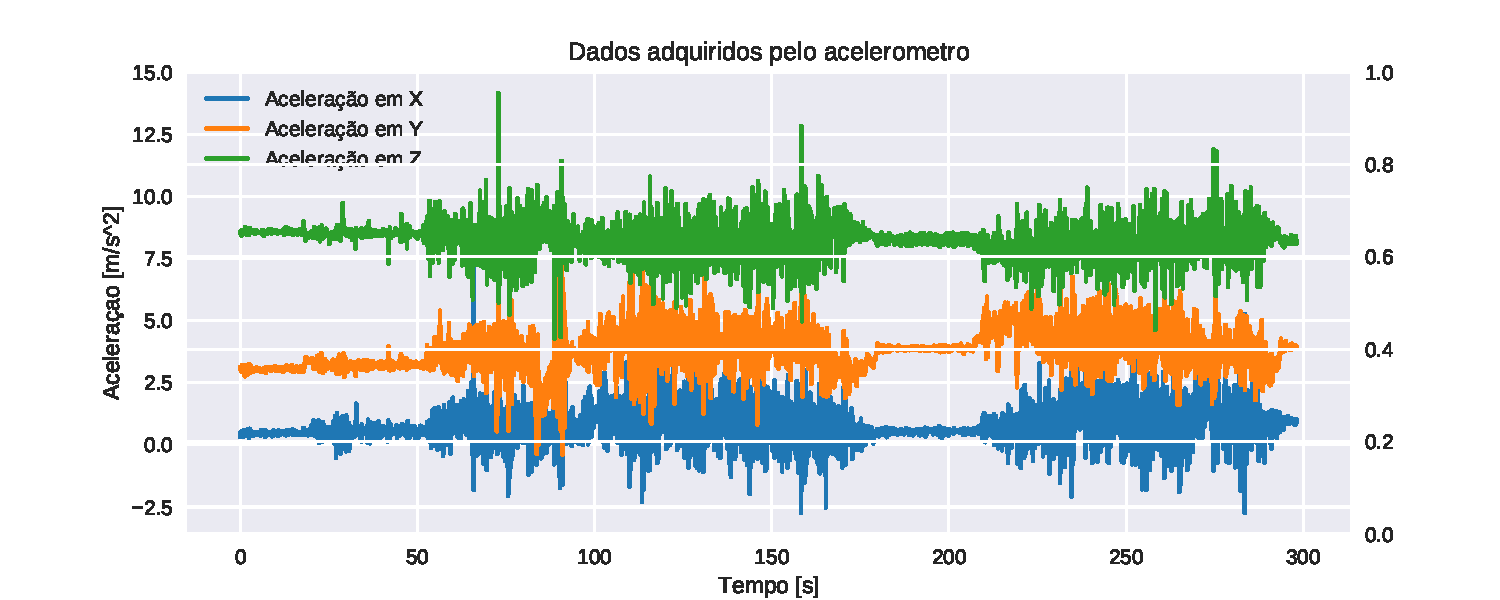
\includegraphics[width=.8\linewidth]{plots/accel_plots.pdf}
    \caption{Exemplo de dados do acelerômetro. Fonte: O autor.}
    \label{fig:raw_accel_plots}
\end{figure}

\begin{figure}[!ht]
    \centering
    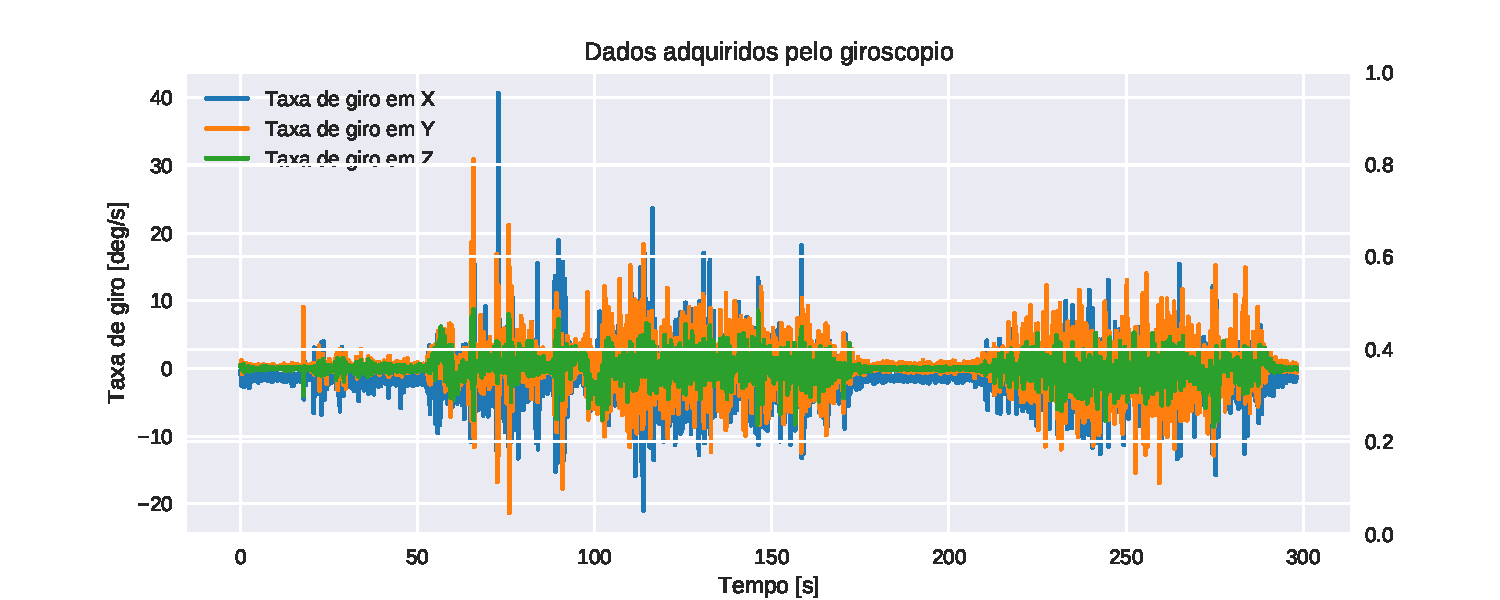
\includegraphics[width=.8\linewidth]{plots/gyro_plots.pdf}
    \caption{Exemplo de dados do giroscópio. Fonte: O autor.}
    \label{fig:raw_gyro_plots}
\end{figure}

\begin{figure}[!ht]
    \centering
    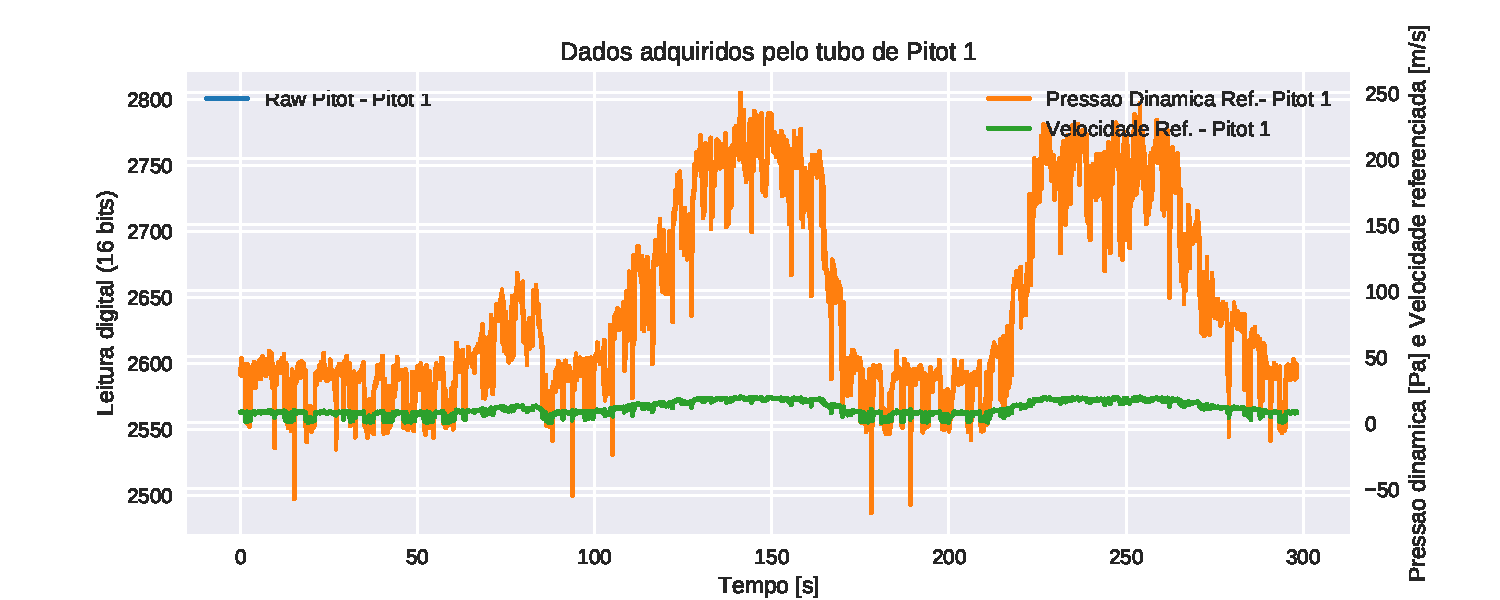
\includegraphics[width=.8\linewidth]{plots/pitot_plots.pdf}
    \caption{Exemplo de dados do Pitot. Fonte: O autor.}
    \label{fig:raw_pitot_plots}
\end{figure}

\begin{figure}[!ht]
    \centering
    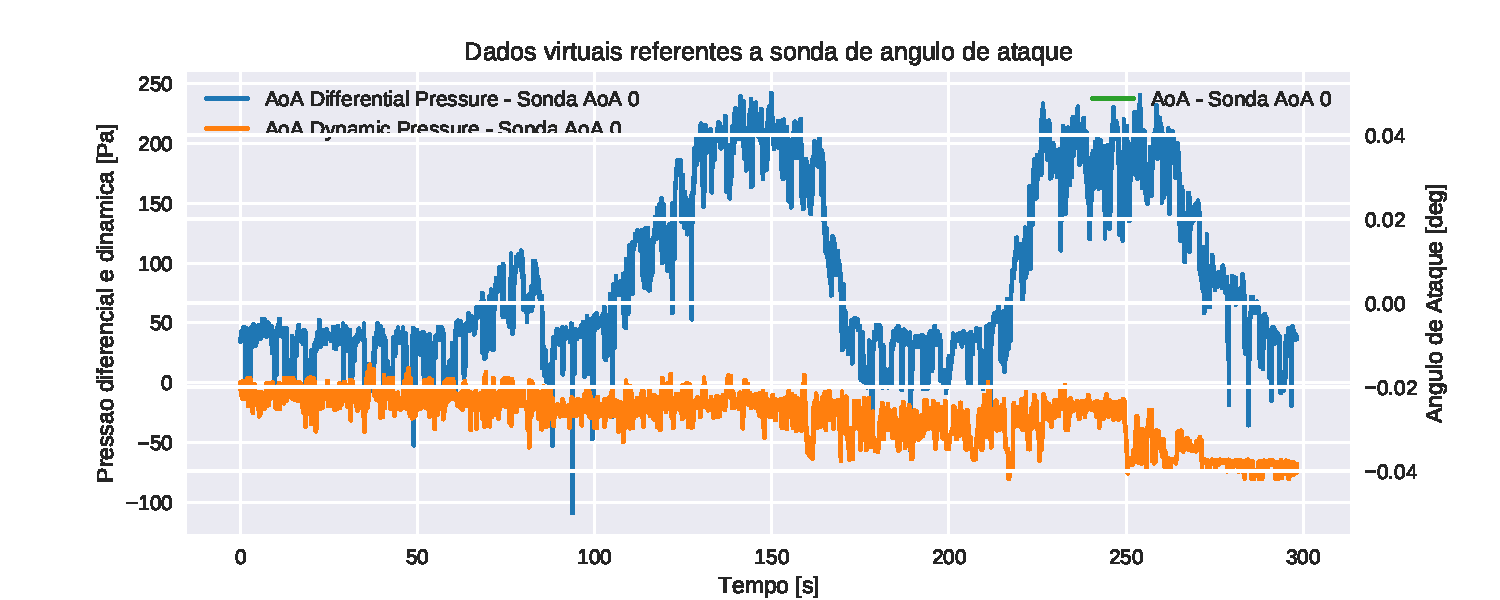
\includegraphics[width=.8\linewidth]{plots/aoa_plots.pdf}
    \caption{Exemplo de dados da sonda de angulo de ataque. Fonte: O autor.}
    \label{fig:raw_aoa_plots}
\end{figure}

\begin{figure}[!ht]
    \centering
    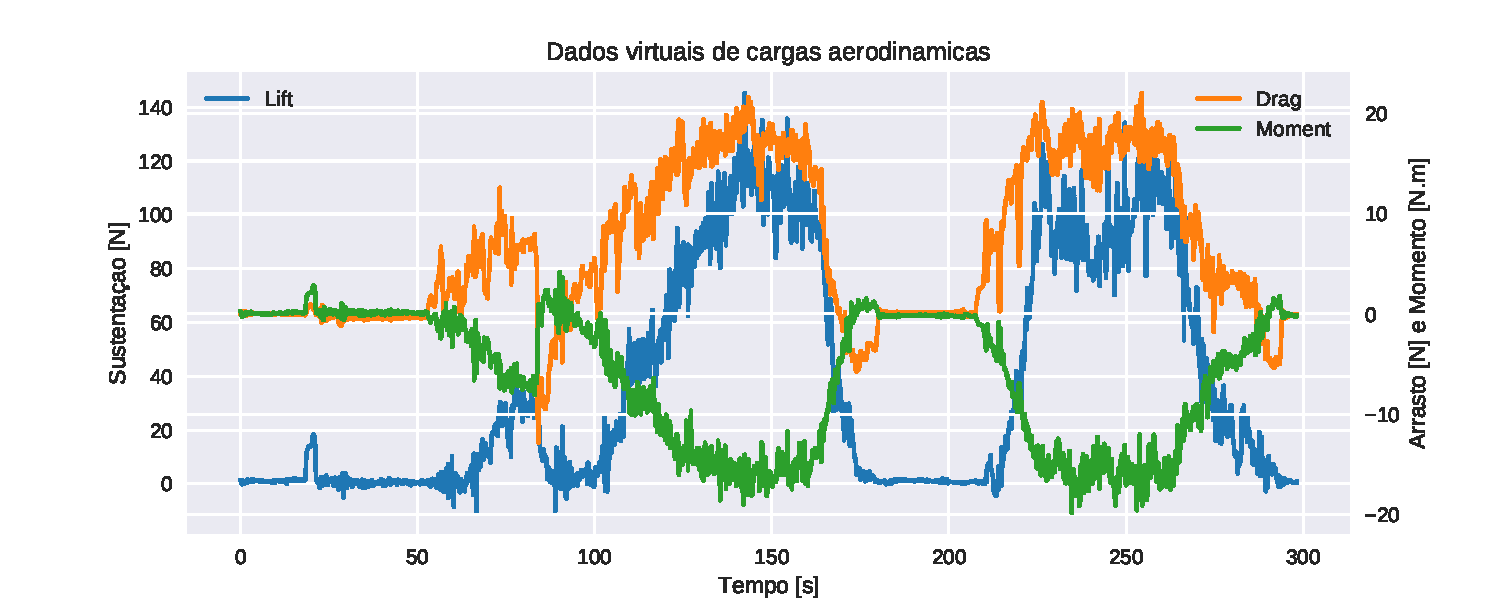
\includegraphics[width=.8\linewidth]{plots/loads_plots.pdf}
    \caption{Exemplo de dados de cargas aerodinâmicas. Fonte: O autor.}
    \label{fig:raw_load_plots}
\end{figure}

\section{Limpeza, filtragem e redução dos dados}

\subsection{Limpeza de dados}

Dado que o teste foi executado procurando-se atingir uma velocidade constante, o resultado final será dado para apenas um valor de Reynolds, sendo assim, dados adquiridos que sejam válidos mas não estejam próximos ao Reynolds do teste não devem ser utilizados, dado que devem apresentar comportamento aerodinâmico diferente daquele correspondente ao Reynolds desejado \citep{anderson1984fundamentals}. Sendo assim, a primeira limpeza a ser realizada é quanto à faixa de interesse de Reynolds. Desta forma os dados a serem utilizados para medição serão aqueles correspondentes aos instantes onde foi alcançada a velocidade estipulada para o teste, com desvio máximo de 10\%.

Para mostrar o resultado desta filtragem usaremos os dados de Sustentação. Os dados originais se encontram na figura \ref{fig:orig_lift_plot} enquanto os dados após filtragem por faixa de Reynolds se encontram na figura \ref{fig:lift_reynolds_filter} :

\begin{figure}[!ht]
    \centering
    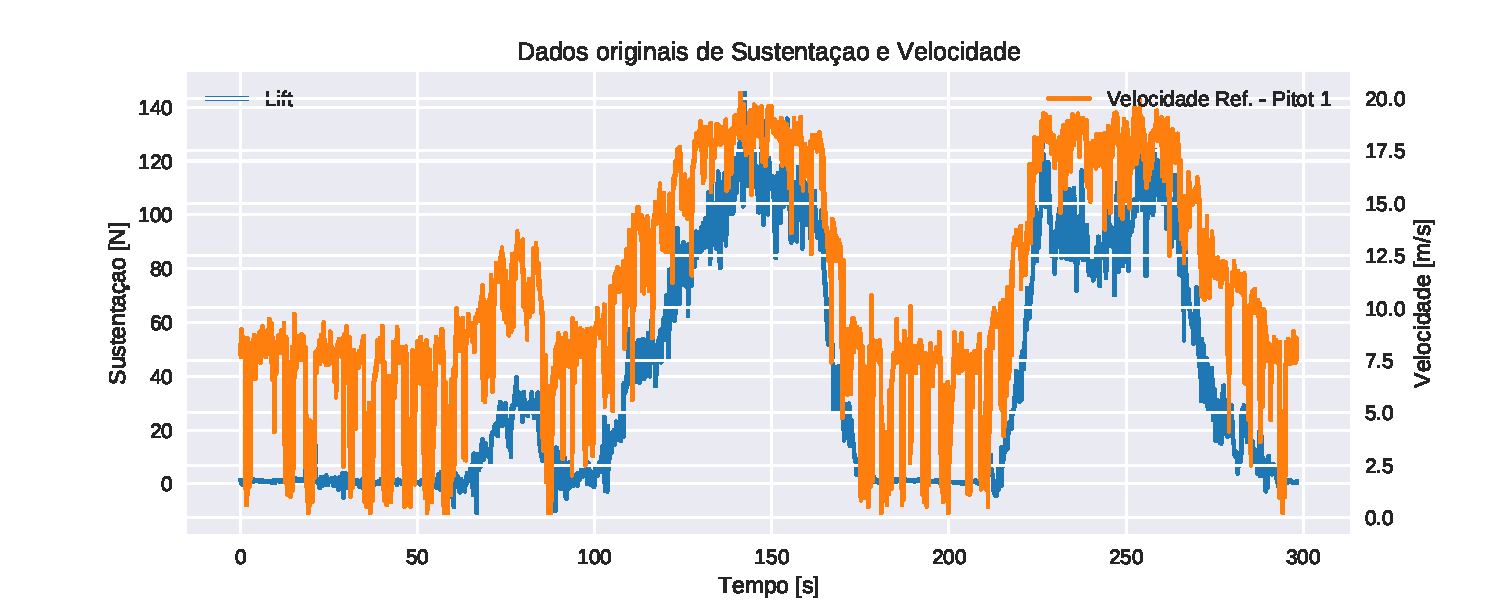
\includegraphics[width=.8\linewidth]{plots/orig_lift_plot.pdf}
    \caption{Dados de sustentação e velocidade originais. Fonte: O autor.}
    \label{fig:orig_lift_plot}
\end{figure}


\begin{figure}[!ht]
    \centering
    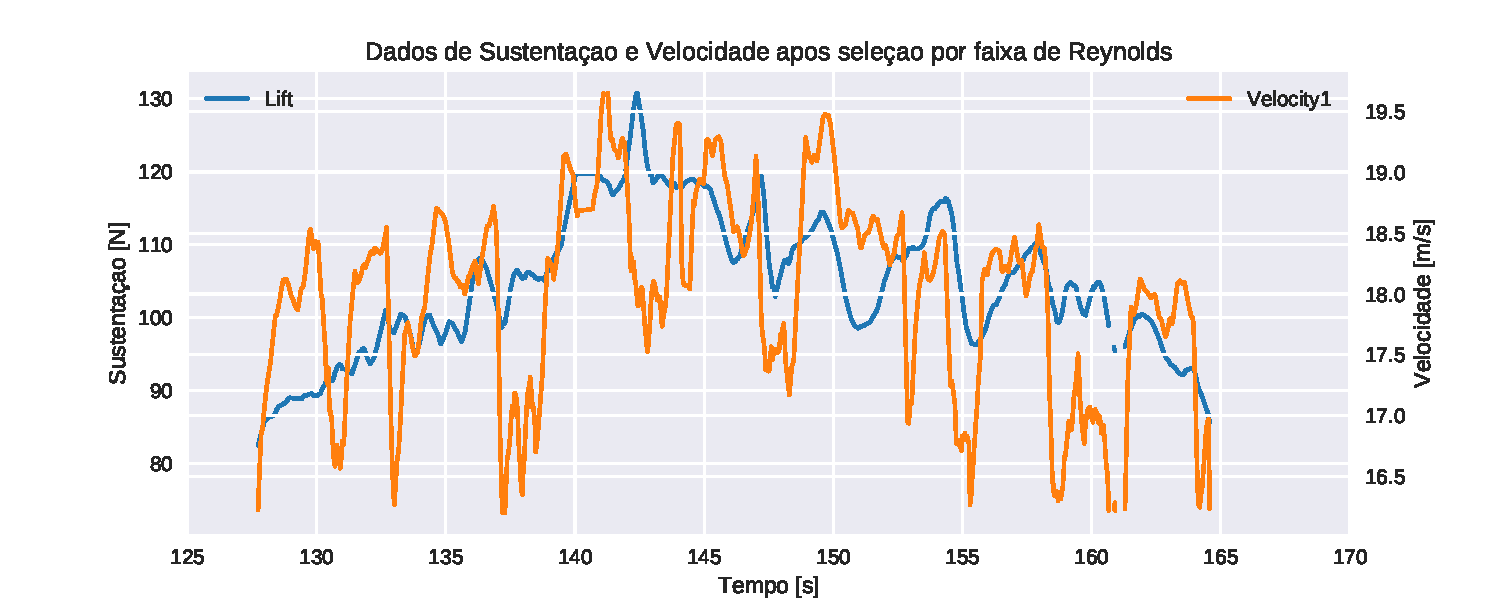
\includegraphics[width=.8\linewidth]{plots/reynolds_lift_plot.pdf}
    \caption{Dados de sustentação e velocidade após filtragem pela faixa de Reynolds do teste (1o patamar). Fonte: O autor.}
    \label{fig:lift_reynolds_filter}
\end{figure}

% A premissa principal para o uso dos dados do teste é de que os valores medidos estejam dentro do intervalo de uso dos sensores e de que as acelerações sobre o sistema sejam baixas. O intervalo de uso dos sensores se encontra na tabela X.

% \begin{table}[!ht]
%     \centering
%     \includegraphics[width=.8\linewidth]{figuras/outras/placeholder.png}
%     \caption{TABELA COM ZONA DE USO DE CADA SENSOR. Fonte: O autor.}
%     \label{fig:placeholder}
% \end{table}

% Após a seleção por faixa de Reynolds, dados fora da faixa de medição dos sensores e dados com aceleração em X, Y ou Z maior que 0.5g foram também descartados.

\subsection{Filtragem}

Após a limpeza dos dados, onde foram removidos aqueles que estavam fora da zona de interesse, buscou-se avaliar a filtragem do sinal, visando aumentar a relação sinal-ruido.

Primeiramente foram realizadas Transformadas Rápidas de Fourier nos dados das células e das sondas de angulo de ataque (incluindo velocidade). Através da transformação para o domínio da frequência foi possível encontrar as frequências de corte ideais para aplicação de filtros passa-baixa em cada um dos dados.

% \begin{figure}[!ht]
%     \centering
%     \includegrapha apoliics[width=.8\linewidth]{figuras/outras/placeholder.png}
%     \caption{ANALISES FFT. Fonte: O autor.}
%     \label{fig:fft_analysis}
% \end{figure}

% A partir do resultado das analises foram dimensionados filtros do tipo passa-baixa para a remoção dos ruídos de alta frequência em cada um dos dados.

% As frequências de corte para cada dado se encontram na tabela X. 

% \begin{table}[!ht]
%     \centering
%     \includegraphics[width=.6\linewidth]{figuras/outras/placeholder.png}
%     \caption{TABELA COM FREQUENCIA DE CORTE DE CADA DADO. Fonte: O autor.}
%     \label{tab:cut_frequency_values}
% \end{table}

A titulo de exemplo, o resultado após filtragem para os dados de sustentação e velocidade se encontram na figura \ref{fig:filtered_lift_plot}.

\begin{figure}[!ht]
    \centering
    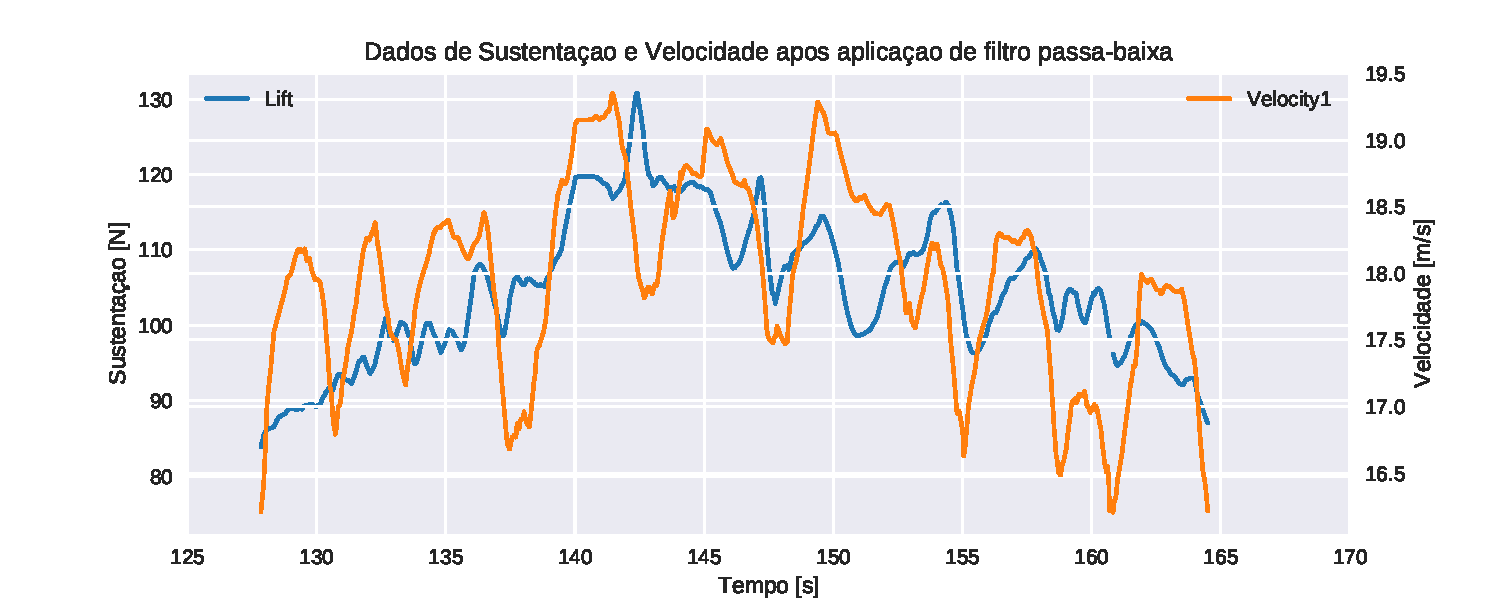
\includegraphics[width=.8\linewidth]{plots/filtered_lift_plot.pdf}
    \caption{Dados de sustentação e velocidade após filtragem das altas frequências. Fonte: O autor.}
    \label{fig:filtered_lift_plot}
\end{figure}

\subsection{Redução}

Em posse dos dados filtrados passa-se à etapa de redução. Não é do interesse do projetista a principio saber qual sustentação, arrasto ou momento foram alcançados durante os testes, pois esses são dados absolutos que dependem do tamanho do componente e da velocidade no instante medido. Para facilidade de analise e mais justa comparação entre diferentes componentes é de interesse a redução destes dados na forma dos coeficientes aerodinâmicos \citep{anderson1984fundamentals}.

\begin{equation}
    C_L =  \frac{L}{ \frac{1}{2} \rho V^{2} S}
    \label{eq:cl}
\end{equation}

\begin{equation} 
    C_D =  \frac{D}{ \frac{1}{2} \rho V^{2} S}
    \label{eq:cd}
\end{equation}

\begin{equation}
    C_M =  \frac{M}{ \frac{1}{2} \rho V^{2} S C_{M.A.}} 
    \label{eq:cm}
\end{equation}

As equações \ref{eq:cl}, \ref{eq:cd} e \ref{eq:cm} foram aplicadas a todas as amostras de dados gerando três novas colunas, $C_L$, $C_D$ e $C_M$, que podem ser visualizadas na figura \ref{fig:coefficients_plot}. Os dados das baterias de testes foram então condensados num mesmo conjunto de dados,para o qual então foram calculados o valor médio e o desvio padrão de cada coeficiente, para cada angulo de incidência.

\begin{figure}[!ht]
    \centering
    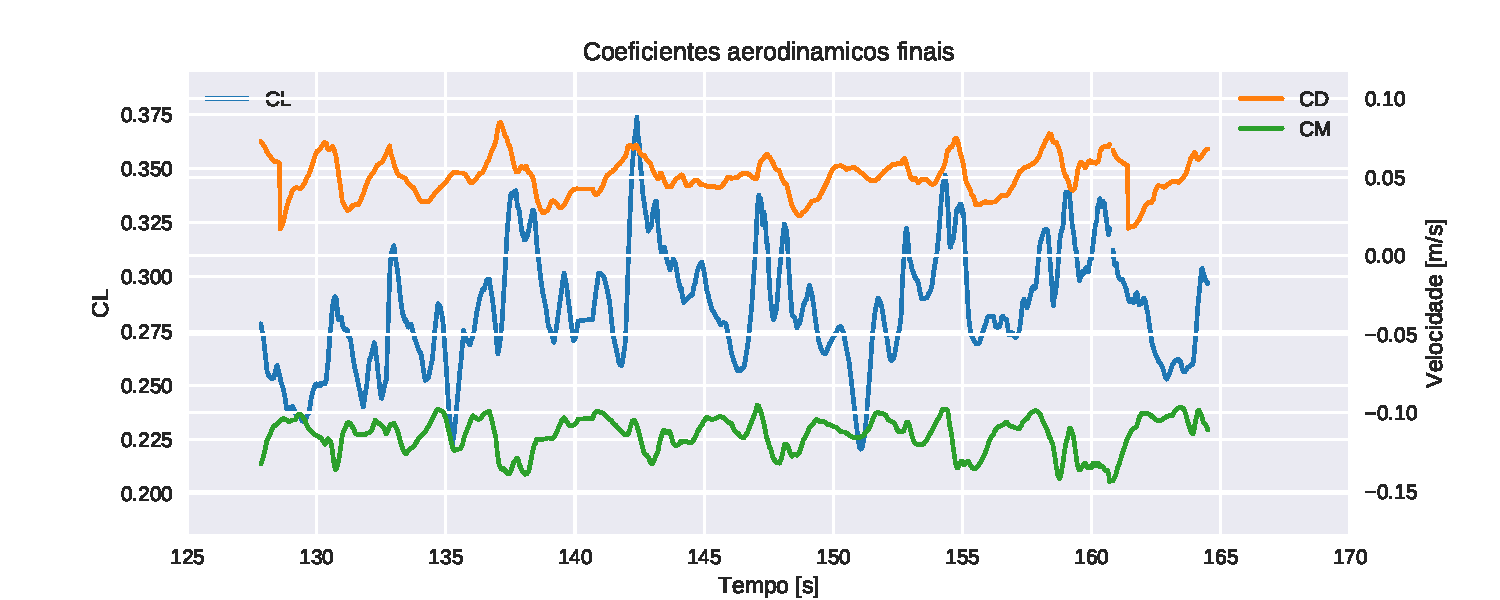
\includegraphics[width=.8\linewidth]{plots/coefficients_plot.pdf}
    \caption{Variação dos coeficientes aerodinâmicos ao longo do tempo para o patamar avaliado. Fonte: O autor.}
    \label{fig:coefficients_plot}
\end{figure}

Os valores finais de media para os coeficientes de cada angulo de incidência estão explicitados nos gráficos da figura \ref{fig:coefficients_alpha_plot}.

\begin{figure}[!ht]
    \centering
    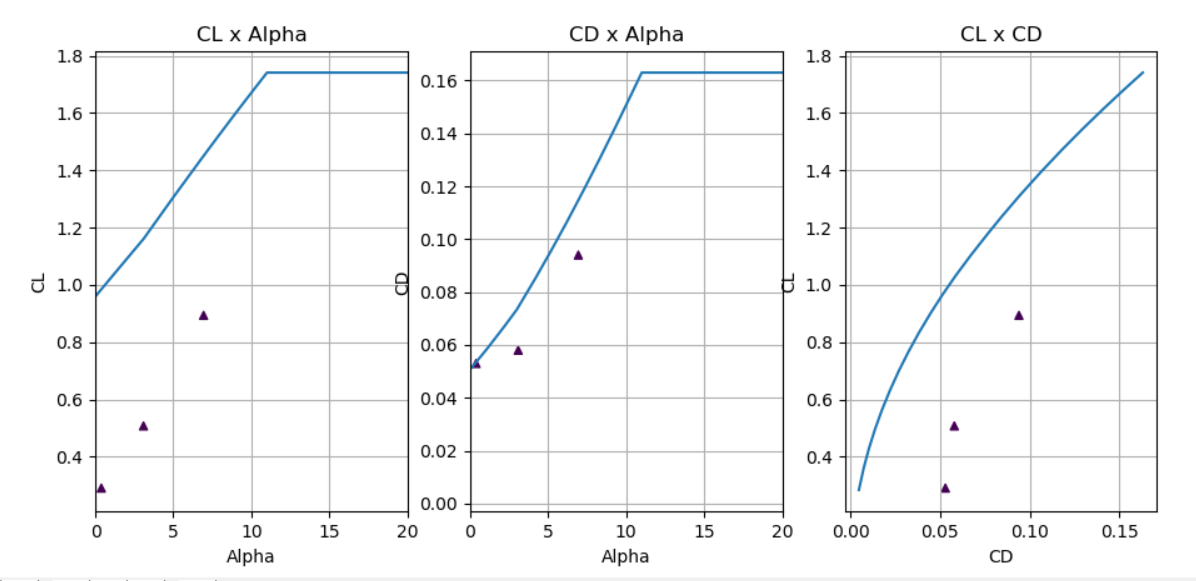
\includegraphics[width=.8\linewidth]{plots/cl_cd_polar_medicao.png}
    \caption{Curvas $C_x vs Alpha$, experimental e simulado. Fonte: O autor.}
    \label{fig:coefficients_alpha_plot}
\end{figure}

Os resultados do teste demonstram um alto desvio entre os valores de sustentação medidos experimentalmente e os simulados. Já os dados de arrasto se encontram próximos entre as duas fontes, porém com os dados experimentais sendo sempre menores que os simulados, ao contrario do que normalmente se espera, dado que os métodos de VLM costumam subestimar o arrasto.

Estes testes se mostraram inconclusivos, indicando apenas que existe pelo menos uma fonte de erro. Este erro pode estar vindo da própria bancada, por alguma falha construtiva ou de calibração, da execução do teste, por exemplo angulando-se o profundor de valor diferente do simulado, ou mesmo do protótipo, por falhas na construção. 

De fato tal aeronave indicou em testes de voo posteriores estar aparentemente com uma relação $C_L/C_D$ mais baixa do que o esperado, não conseguindo decolar com cargas maiores que 70\% daquela estimada em projeto, além de apresentar assimetria de sustentação entre os dois lados da asa, indicando diminuição da sustentação total gerada com relação aquela estimada em projeto.

Além disso os dados coletados aparentaram boa qualidade e relativa estabilidade, além de apresentarem comportamento coerente com o esperado. Erros na angulação do profundor, mesmo que altas, também não acarretariam em desvio tao grande dos valores de sustentação. Deste modo, parece provável um desvio do próprio protótipo em relação ao simulado, porém é importante que fique claro que tal hipótese não pode ser comprovada, dado que a bancada não foi validada contra valores conhecidos de literatura.


 % Texto do cap4.tex
\chapter{Conclusão}\label{chp:conc}

    Este trabalho procurou descrever o projeto, construção e teste de uma bancada experimental para caracterização aerodinâmica de componentes de VANTs, visando eliminar a necessidade de testes em túnel de vento ou ensaios em voo.
    
    O trabalho foi desenvolvida no âmbito de uma equipe de projeto aeronáutico, buscando preencher a necessidade da mesma por dados experimentais que norteassem a validação e otimização de seus projetos.
    
    O trabalho foi bem sucedido no sentido de projetar, construir e testar tal bancada, cumprindo os requisitos estabelecidos de custo, facilidade de uso, desenvolvimento de softwares de suporte e documentação. 
    
    Os resultados obtidos no teste estão dentro do esperado quando comparados as simulações para os mesmos componentes testados.  Não foram testados contudo componentes com valores experimentais conhecidos, de forma que não se pode dizer que a bancada esta validada. Esperava-se ao inicio deste trabalho validar ou invalidar a bancada, porém a necessidade de finalizar os ensaios experimentais antes do previsto impediu que tal ação fosse concluída.
    
    Durante o desenvolvimento deste trabalho, dificuldades surgiram onde se poderia e onde não se poderia imaginar. Atrasos na entrega dos componentes, cargas não previstas, erros na execução dos testes, comportamentos inesperados do software de aquisição de dados, comportamentos inesperados dos sensores, todos foram problemas encontrados durante o caminho, felizmente resolvidos, um a um, ainda que atrasando o cronograma previsto.
    
    O uso da bancada hoje se encontra bastante facilitado, sendo possível realizar os testes e a analise dos resultados em uma noite de trabalho, considerando um bom planejamento e execução dos mesmos.
    
\section{Trabalhos futuros}
    
    Pode-se dizer que este trabalho se encontra em estagio avançado, mas ainda não concluído. A principal necessidade que se enxerga para um trabalho futuro é a validação da mesma para componentes já experimentalmente caracterizados. Esta validação agregaria em muito e permitiria que a equipe Céu Azul passasse a realizar seus ensaios experimentais visando otimizar o projeto com uma maior garantia sobre a validade dos resultados. Além da própria validação, alguns pontos a se tratar no futuro, seja por este autor ou por um terceiro, são levantados:
    
\begin{itemize}
    \item Mudança na solução da bandeja inferior da balança, passando a utilizar 3 células de carga e eliminando as guias lineares.
    \item Calibração dos fatores de acoplamento entre medições de sustentação e arrasto
    \item Validação da bancada contra geometrias com valores experimentais já consolidados, tais como esferas, cilindros e asas de perfil NACA
    \item Desenvolvimento de interface gráfica para carregamento dos dados de testes, visando eliminar a necessidade de execução das analises via scripts.
    \item Inclusão de rotina de calibração das células de carga e dos tubos de Pitot via app, tornando a calibração um processo rápido e facilitado.
    \item Inclusão de rotina de testes de forma guiada pelo app, isto é, em um formato de passo-a-passo, com instruções de execução, avisos de mal-uso ou resultados inconsistentes e automatização das analises.
    \item Possibilidade de transferência dos dados da plataforma de aquisição para o celular via Bluetooth, eliminando a necessidade de retirada do cartão de memoria da mesma.
    \item Inclusão de modo de gravação de áudio no app, visando a possibilidade de uma "narração" do teste pelo responsável. Este áudio permitiria que avaliações extras pudessem ser realizadas pelo responsável pela analise, como identificação de possíveis erros de execução, anormalidades ou mesmo testes diferenciados, como a execução de comandos na aeronave a serem posteriormente caracterizados. 
\end{itemize}
 % Texto do cap5.tex



%%%%%%%%%%%%%%%%%%%%%%%%%%
%%Elementos Pós-Textuais%%
%%%%%%%%%%%%%%%%%%%%%%%%%%
%%--------Bibliografia--------
\Bibliografia{referenciasbibliograficas} % arquivo bibtex com as referências (referenciasbibliograficas.bib)

%%--------Apêndice--------
%% Descomente caso exista a necessidade da inclusão de apêndices
%\apendice % Comando que inclui os apêndices
%\include{7_Apendice/apendice_1}   % Arquivo apendice_1.tex
%\include{7_Apendice/apendice_2}   % Arquivo apendice_2.tex
%%---------------------------------------------------------------

%%--------Anexos-------------------------------------------------
%% Descomente caso exista a necessidade da inclusão de anexos
%\anexo % Comando que inclui os anexos (outros autores)
%\include{8_Anexos/anexo_1}  % Arquivo anexo_1.tex
%\include{8_Anexos/anexo_2}  % Arquivo anexo_2.tex
%%---------------------------------------------------------------

\end{document}
